\subsection{Modelli ad Agente}
% scrivere sezione simile ad articolo (download)
Un modello ad agente è un modello computazionale per la simulazione delle 
azioni e interazioni di un insieme di agenti autonomi, siano essi individui
o gruppi di individui, con l'obiettivo di comprendere il comportamento 
del sistema e la relazione che vige con i suoi risultati \cite{wiki:Agent-based_model}
\cite{7822080}.

Nella modellazione basata su agenti, un sistema viene modellato come un insieme 
di entità decisionali autonome chiamate \emph{agenti}. Ogni agente valuta 
individualmente la propria situazione e prende decisioni sulla base di un insieme di 
regole ben precise. Gli agenti possono eseguire diversi comportamenti appropriati
al sistema che rappresentano. Interazioni competitive e ripetute tra agenti sono 
peculiarità di un modello ad agente che si basa sulla potenza computazionale di un 
computer per esplorare dinamiche che altrimenti non sarebbero esplorabili tramite la 
classica modellazione matematica. Nella sua rappresentazione più semplice, un modello 
ad agente consiste in un sistema di agenti e relazioni tra loro, e questo permette 
perfino a un modello estremamente semplice di mostrare comportamenti complessi e 
permette di ottenere informazioni preziose riguardo le dinamiche del mondo reale che
modellano. 

Generalmente un agente può essere capace di \emph{evolvere} nel tempo, permettendo 
di osservare comportamenti precedentemente inaccessibili, denominati \textbf{comportamenti emergenti}.
I modelli più sofisticati incorporano generalmente reti neurali, algoritmi evolutivi o 
altre tecniche di apprendimento per premettere alla simulazione di essere quanto più 
realistica possibile.

L'utilizzo di modelli ad agente in epidemiologia è una tecnica nota che 
da più di un decennio viene impiegata per simulare e comprendere 
i problemi più disparati, tutti però generalmente accomunati
dal fatto che come parametro portante vi sia il comportamento umano \cite{Groff2019}
\cite{El-Sayed2012-ac} \cite{Tracy2018-lc} \cite{Bissett2021}. 
Uno dei parametri più caratterizzanti che da sempre sono stati tenuti 
in considerazione e assunti come ristretti ad una piccola cerchia, sono 
le interazioni sociali tra individui. Questo sovrainsieme di parametri 
racchiude molteplici sottoinsiemi di parametri che descrivono delle 
interazioni più specifiche ma che possono essere raggruppate come macro 
categoria se si scende a compromessi. 

\begin{minipage}{\linewidth}
    \centering
    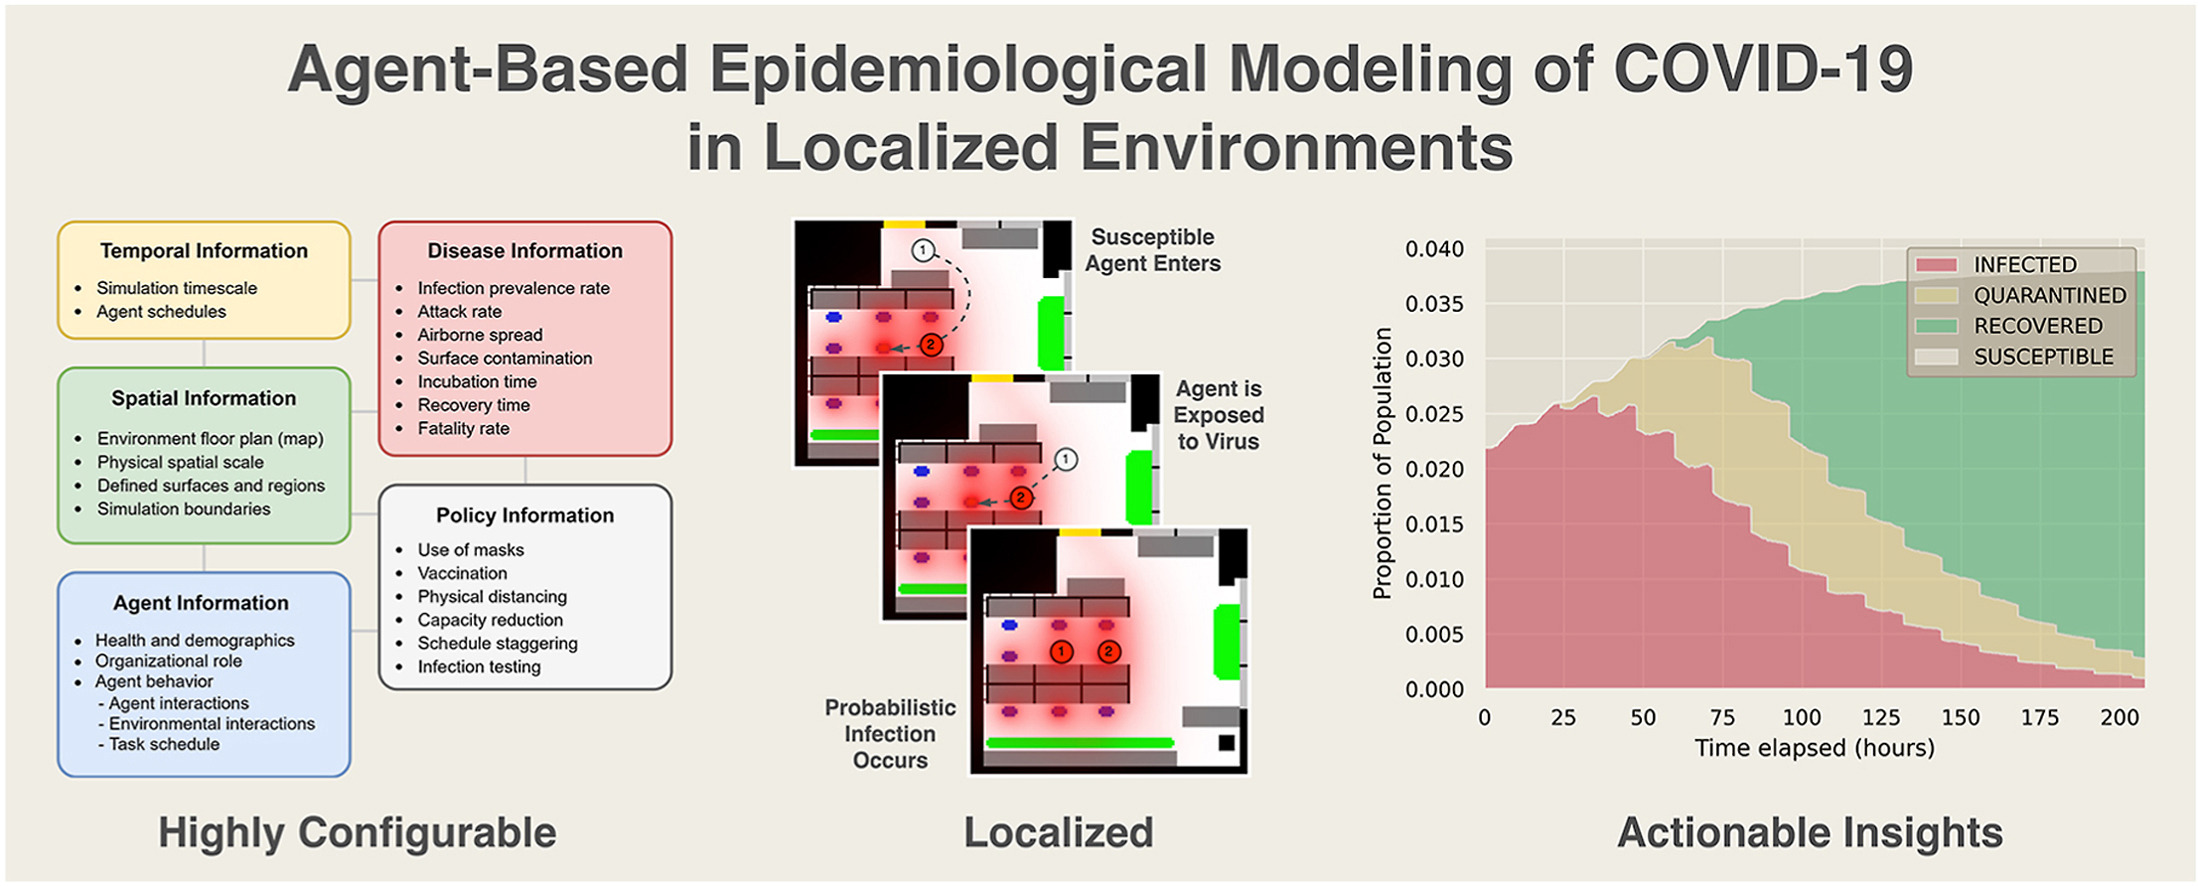
\includegraphics{img/1-s2.0-S0010482522001883-ga1.jpg}
    \captionof{figure}{Agent-Based Epidemiological Modeling of COVID-19 in Localized Environment \cite{CIUNKIEWICZ2022105396}}
    \label{fig:abm_covid}
\end{minipage}

Questa specifica è importante in quanto uno delle sfide più grandi che 
il mondo della simulazione, e quindi quello epidemiologico devono affrontare
è proprio quello di trovare un modo efficiente e soprattutto realistico 
di simulare le interazioni sociali tra individui, in quanto queste possono
influenzare notevolmente i risultati di una simulazione definendola utile
oppure inutile \cite{Silverman2021}. Non soltanto, un'altra sfida è il modo 
con cui si decide di rappresentare lo spazio (e il tempo) all'interno della
simulazione. In base al tipo di discretizzazione effettuata una simulazione
potrebbe essere utile in un campo ma totalmente inutile in un altro 
\cite{KONSTANTINOUDIS2020100319}.

I vantaggi di utilizzare una tecnica di simulazione tramite modello ad agente
sono principalmente i seguenti:
\begin{itemize}
    \item I modelli ad agente riescono a catturare molto bene i comportamenti emergenti
    \item I modelli ad agente forniscono una descrizione naturale del sistema che rappresentano 
    \item i modelli ad agente sono \emph{flessibili}
\end{itemize}
è chiaro come principalmente la scelta dell'utilizzo di un modello di simulazione viene preferito 
sopra le altre tecniche di simulazione è proprio per via della possibilità di catturare i 
comportamenti emergenti del sistema.

\begin{minipage}{\linewidth}
    \centering
    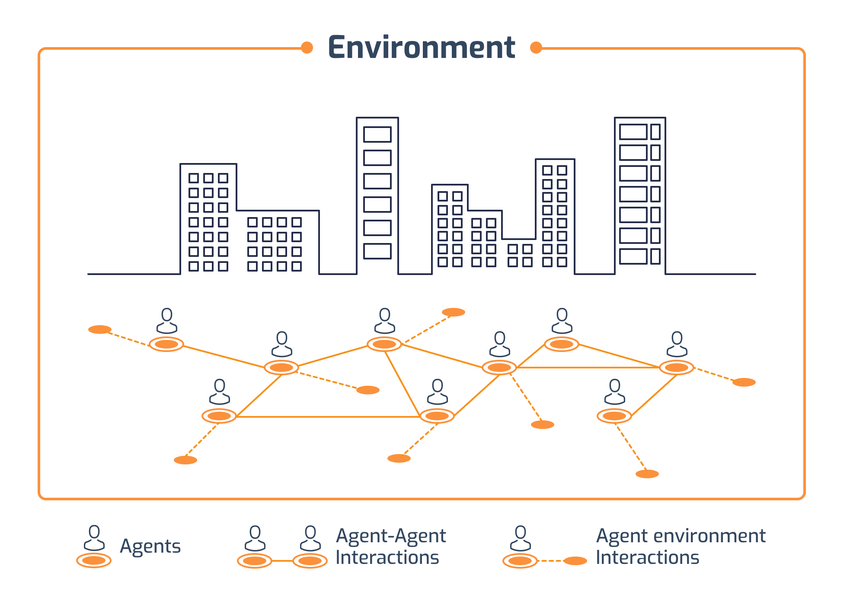
\includegraphics[scale=0.5]{img/Schematic-representation-of-an-agent-based-model-ABM.png}
    \captionof{figure}{Rappresentazione schematica di un modello ad agente}
    \label{fig:schematic_representation_abm}
\end{minipage}

Con l'arrivo della pandemia da COVID-19 molti ricercatori hanno 
focalizzato la propria attenzione sull'idea di sviluppare un modello 
ad agente puro oppure ibridato \cite{Marzban2021-pd} con delle equazioni
differenziali, con l'obiettivo di 
trovare un modello di simulazione in grado di simulare in maniera 
affidabile il decorso di una pandemia tenendo in considerazione le 
variabili più stocastiche e imprevedibili come il comportamento umano, e 
magari ottenere un intuizione riguardo il comportamento emergente del sistema.

\subsubsection*{Comportamento emergente}
I fenomeni emergenti sono il risultato dell'interazione di entità individuali. 
Per definizione non possono essere ridotte ad una parte del sistema in quanto 
l'insieme del sistema è maggiore della somma delle sue singole parti, questo poichè 
si deve tenere in considerazione le interazioni tra le parti. Un comportamento emergente 
può avere proprietà che sono separate dalle proprietà intrinseche delle parti.
Per questo motivo i comportamenti emergenti rendono complesso lo studio e l'analisi del
sistema, in particolare rendono difficile predirne il comportamento, in quanto questi comportamenti 
possono essere controintuitivi. 

\begin{minipage}{\linewidth}
    \centering
    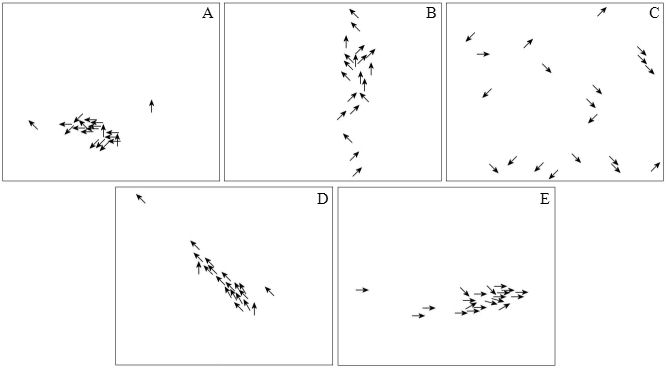
\includegraphics{img/Figure6b.jpg}
    \captionof{figure}{Esempio di comportamento emergente nella simulazione degli stormi di uccelli}
    \label{fig:flock_emergent_behaviour}
\end{minipage}

è interessante notare come un modello ad agente generi un comportamento emergente dal basso 
verso l'alto ovvero dai singoli agenti fino all'intero gruppo, e questo alza un interrogativo 
su cosa possa costituire un comportamento emergente. 

\subsubsection{Discretizzazione}
La tematica della discretizzazione è una delle proprietà fondamentali
e al contempo uno dei problemi atavici della simulazione.
Il mondo in cui viviamo è un mondo continuo, ma gli strumenti
che attualmente abbiamo per simularlo sono discreti, per cui 
ogni qualvolta che vogliamo simulare un evento dobbiamo decidere 
in che modo adattare la realtà alla simulazione, andando 
inequivocabilmente a perdere informazioni nel processo 
\cite{KONSTANTINOUDIS2020100319}. 

Il processo di discretizzazione in una simulazione può prendere 
principalmente due macro aree che sono: lo spazio e il tempo. 
Molti framework di simulazione implementano al loro interno 
diversi trucchetti per simulare in maniera quanto più accurata
un insieme di dati continuo, permettendo all'utente di utilizzare
parole chiave come ad esempio \textbf{ContinuousSpace}. Quello che praticamente
viene fatto è creare un ambiente per il modello che è il più
preciso e granulare possibile in maniera tale da avere una descrizione
quanto più accurata (anche se imprecisa) del mondo. 

Il processo di discretizzazione comunque non è sempre negativo, 
in quanto alcuni problemi possono essere simulati in maniera 
estremamente fedele anche effettuando questi accorgimenti, e anzi
alle volte non è perfino necessario avere una precisione troppo 
alta per la simulazione di determinati eventi.

\begin{minipage}{\linewidth}
    \centering
    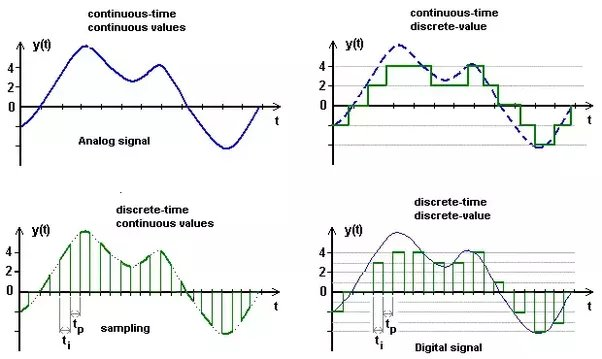
\includegraphics[scale=0.5]{img/main-qimg-100fc99cfe855462247225a07e1dfb7e-pjlq.jpg}
    \captionof{figure}{Esempio di differenti tipologie di discretizzazione, siano esse nel tempo o nei valori}
    \label{fig:discretization}
\end{minipage}
